\chapter{Aquifer test - Equipment}
\label{chapter:fieldwork_set-up}

The northern Ghana in-field geohydrological data collection would not have been possible without the interference of Conservation Alliance (CA). Spread over the Upper East and Northern Region the NGO holds multiple PIT locations. Five locations, visible in figure \ref{fig:Overviewlocations}, are appointed as measurement locations for the purposes of this research.
Besides the research locations, CA provided transport, an interpreter and pumping test equipment. The section below contains detailed information on the equipment applied. A distinction has been made between the equipment for the pumping tests and the actual groundwater measurements. Moreover small equipment as pliers, screwdrivers, gloves and robes are ignored. Purposes and use of these tools are taken for granted.\\
% Moreover, it describes the general fieldwork pumping test / monitoring set-up. The section concludes with fieldwork fact-sheets, containing the collected data for each individual location. 
%The applied in-field pumping tests are executed with a same set of equipment. The paragraph below contains a detailed description of the most important tools. In this case a distinction has been made between the equipment for the pumping tests and the actual groundwater measurements. Moreover small equipment as pliers, screwdrivers, gloves and robes are ignored. Purposes and use of these tools are taken for granted. \\

\section{Pumping test} 

\begin{itemize}
\item Pump: Pedrollo 4” submersible pump; Type 4SR4/18 \\
A 2 HP pump, for example usable for the supply of water to irrigation fields. While pumping the water should preferably not exceed 35 $^{\circ}$C and should not contain too many particles; no more than 150 g/m$^{3}$. The pump can be submerged in water up to 100 meters. Installed in the right way, the pump can deliver 20-100 l/min with an head difference of 112-45 m. More specific information regarding the pump can be found on the Pedrollo webpage.

\begin{figure}[h!]
 \centering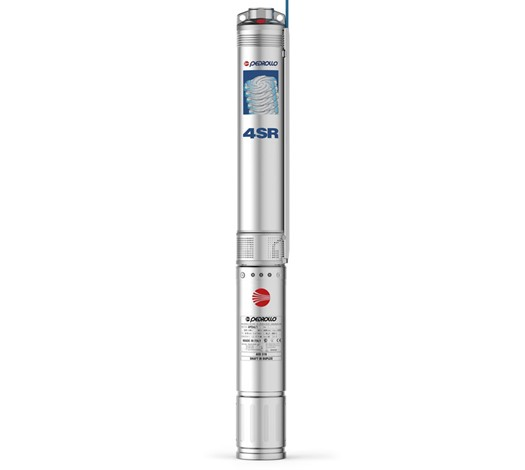
\includegraphics[width=0.35\linewidth]{Pedrollo}
 \captionsetup{justification=centering}
 \caption[Comparable example of the fieldwork submersible pump]{Comparable example of the fieldwork submersible pump \\ (source: \url{https://www.pedrollo.com/en/4sr-4-submersible-pumps/150})} 
 \label{fig:Pedrollo}
\end{figure}

\item Generator \& power converter: Kipor diesel generator - 5 kVA \\
A mobile generator has been used as a pump power source. The Kipor generator is a relatively small model, easy to handle and meets the pump requirements by the use of the 230 V connection. A power converter is placed between generator and pump to manually switch on and off the pump. To facilitate a flawless transfer between generator and pump one should be aware the cables and connections towards the pump should be waterproof. Moreover these power cables should be of a decent length to allow the pump to submerge. 

\begin{figure}[h!]
 \centering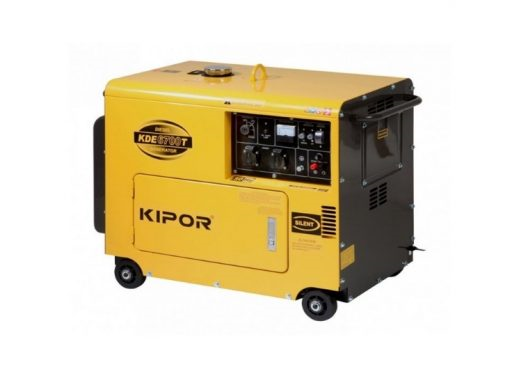
\includegraphics[width=0.40\linewidth]{Kipor}
 \captionsetup{justification=centering}
 \caption[Comparable example of the fieldwork generator]{Comparable example of the fieldwork generator \\ (source: \url{https://www.kipor-power.eu/winkel/kipor-kde6700t-diesel-generator-5-kva/})}
 \label{fig:Kipor}
\end{figure}

\item Hose: \\
As a transport line towards the location of discharge a flexible water hose has been attached to the pump. The hose has been manufactured in Polyethylene, has an external diameter of 1$^{1⁄4}$” and is approximately 100 m long. 

\begin{figure}[h!]
 \centering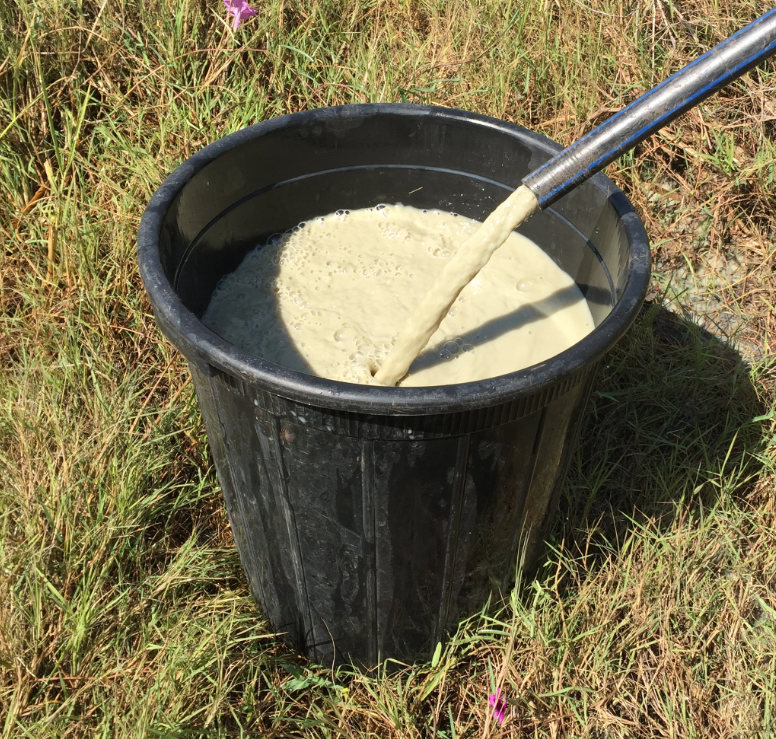
\includegraphics[width=0.35\linewidth]{Hosebucket}
 \captionsetup{justification=centering}
 \caption{Actual fieldwork hose \& bucket}
 \label{fig:Hosebucket}
\end{figure}

\item Bucket: \\
As a rough estimation for discharge an  plastic bucket has been used. This oversized measuring cup stores volumes up to 50 l and contains 5 l level indicators. 

\end{itemize}

\bigskip
\section{Water table monitoring} 

\begin{itemize}
\item Pressure sensor data loggers: \\
\-- Van Essen; TD-Diver Type DI801 (2x) \& Baro-Diver Type DI800 (1x):\\
TD- and Baro-Divers are applied for the measuring and recording of time dependent fluctuations in (ground)water levels, atmospheric pressures and temperatures. The TD-Divers can record a water column up to 10 m. Baro-Divers can be used to measure atmospheric pressures and shallow water levels, approximately up to a range of 0.9 m. Based on the internal memory these devices can store up to 72.000 measurements per parameter. Measurement logging can be programmed by the use of a USB-Unit and the Diver-Office software. With a battery life of 10 years, long and/or short term measurements can be applied with a sample interval of 0.5 seconds to 99 hours. Moreover the sample interval can be linear or logarithmic.

\begin{figure}[h!]
 \centering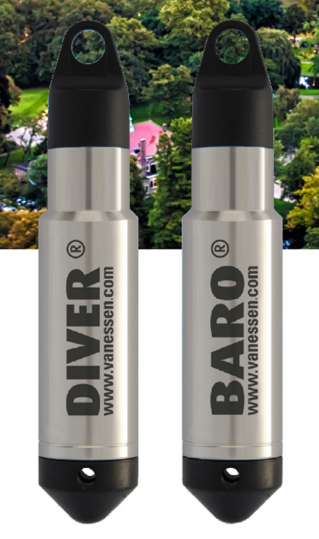
\includegraphics[width=0.17\linewidth]{Essen}
 \captionsetup{justification=centering}
 \caption[Comparable examples of Van Essen TD- \& Baro-Divers]{Comparable examples of Van Essen TD- \& Baro-Divers \\(source: \url{https://www.vanessen.com/images/PDFs/TD-Diver-DI8xx-ProductManual-nl.pdf})}
 \label{fig:Essen}
\end{figure}

\-- In-Situ; RuggedTROLL100 (2x) \& BaroTROLL (1x):\\
Rugged TROLL 100 and BaroTROLL divers are applied for the measuring and recording of time dependent fluctuations in (ground)water levels, atmospheric pressures and temperatures. The RuggedTROLL100 divers function in a pressure range up to 9 m water column. BaroTROLL divers can be used for the measurement of atmospheric pressures, up to 1 bar. The internal memory of 2.0 MB accommodates the storage of 120.000 data records. A record contains a set of three items; date \& time, pressure and temperature. The internal battery has a lifetime of approximately 10 years. By the use of the Rugged TROLL docking-station and the Win-Situ 5 software, linear logging can be programmed. Fastest logging rate is 1 log per second for the Rugged TROLL 100 divers and 1 log per minute for the BaroTROLL divers. Optionally it is possible to display the pressure in units of Psi, Bar, Pascal or mH$_{2}$O. 

%More information on the In-Situ RuggedTROLL100 and BaroTROLL can be found online: \href{https://www.in-situ.com/wp-content/uploads/2014/11/SS\_RuggedTROLL\_100\_200\_Dec2017.pdf}{https://www.in-\\situ.com/wp-content/uploads/2014/11/SS\_RuggedTROLL\_100\_200\_Dec2017.pdf}. (dit laatste tussen de kromme haakjes) is de text die wordt gedisplayed)

\begin{figure}[h!]
 \centering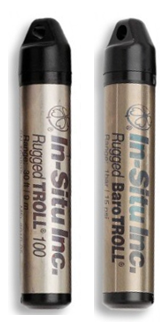
\includegraphics[width=0.17\linewidth]{TROLL}
 \captionsetup{justification=centering}
 \caption[Comparable examples of In-Situ TD- \& Baro-Divers]{Comparable examples of In-Situ TD- \& Baro-Divers \\ (source: \url{https://in-situ.com/product-category/water-level-monitoring/level-temp-data-loggers/})}
 \label{fig:TROLL}
\end{figure}
% hier met \\ een eigen cut-off naar volgende lijn gemaakt, waarbij de ref blijft werken

\item Hand measurement device: Heron water tape \\
The water tape is applied to hand measure static water levels and verify drawdown water levels during the pumping tests. The water tape has a length of 300 ft (100 m). A water level sensing probe is attached to the tail of the tape. Probe water contact results in an instant auditory signal, after which the depth can be determined by eye. Product specifications can be found on the Heron webpage.

\begin{figure}[h!]
 \centering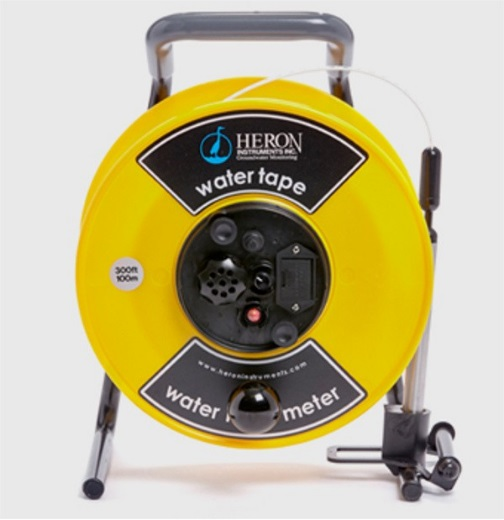
\includegraphics[width=0.35\linewidth]{Heron}
 \captionsetup{justification=centering}
 \caption[Comparable example of the fieldwork water tape]{Comparable example of the fieldwork water tape \\ (source: \url{https://envirotechonline.com/water-level-interface-meters/the-heron-water-tape.html})}
 \label{fig:Heron}
\end{figure}

\end{itemize}